\section{Bài toán tạo sinh chuỗi}

Có rất nhiều cách để tạo sinh chuỗi từ mạng RNN (Recurrent Neutral Network) đã được huấn luyện trước, có thể kể đến như là: Greedy Search, Bean Search, Random Sampling. Nhưng trong đó Random Sampling là một trong những cách có tính ứng dụng cao nhất. Trong phạm vi chương này chúng ta chỉ tìm hiểu về cách tạo sinh chuỗi bằng phương pháp Radom Sampling. Bạn đọc có thể tìm hiểu hai cách còn lại tại Daniël Heres' website [\ref{refer:20}].

\subsection{Tạo mẫu từ phân bố xác suất bất kì}
Tạo mẫu bất kì từ một phân bố xác suất cho trước là một bước quan trọng trong bài toán tạo sinh chuỗi. Như chúng ta đã biết từ các chương trước, đầu ra của mạng RNN là một phân bố xác suất rời rạc, bởi vì hàm softmax được kích hoạt ở tầng cuối của mạng. Từ các phân bố xác suất này chúng ta phải chọn ra những từ phù hợp với từng xác suất của nó. Để làm được điều đó, chúng ta cần tìm hiểu hai khái niệm: tạo mẫu từ phần bố đều và hàm phân phối tích lũy.

Phân bố đều (uniform distribution) là phân bố có biến ngẫu nhiên nhận giá trị trên đoạn $[a, b]$. Xác xuất $X$ nhận bất kỳ giá trị nào thuộc khoảng $[a, b]$ đều bằng $\frac{1}{b-a}$. Chính tính chất này nên phân bố đều được áp dụng để phát sinh số ngẫu nhiên, đảm bảo các giá trị được sinh ra đều các khả năng như nhau.

Hàm phân phối tích lũy (cumulative distribution function - $cdf$) là hàm mô tả đầy đủ phân phối xác suất của biến ngẫu nhiên có giá trị thực $x$. Với mỗi số thực $x$, $cdf$ được định nghĩa như sau:
\begin{align*}
  F(x) &= P(X <= x)
\end{align*}

trong đó vế phải biểu diễn xác suất mà biến ngẫu nhiên $X$ lấy giá trị nhỏ hơn hay bằng $x$. Để hiểu rõ hơn về $cdf$ chúng ta cùng xem ví dụ sau. Giả sử chúng ta có phân bố xác suất của các từ cần phát sinh là.
\begin{align*}
  P(x) &= [0.2, \, 0.01, \, 0.02, \, 0.1, \, 0.05, \, 0.07, \, 0.05, \, 0.5]
\end{align*}

với mỗi xác suất trong $P$ tương ứng với các từ 
\begin{align*}
  ["Hom", \, "nay", \, "toi", \, "di", \, "hoc", \, "Ngay", \, "mai", \, "cung"]
\end{align*}

Hàm phân phối tích lũy của ví dụ trên được tính và có dạng như hình dưới đây.
\begin{align*}
  F(x) &= [0.2, \, 0.21, \, 0.23, \, 0.33, \, 0.38, \, 0.45, \, 0.5, \, 1.0]
\end{align*}

\clearpage
\begin{figure}[h!]
	\centering
		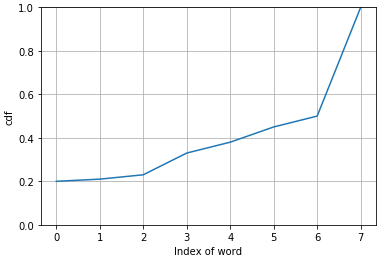
\includegraphics[width=0.6\columnwidth]{chapter07/figure-sec3/cdf.jpg}
		\centering
	\caption{Hàm phân phối tích lũy của các từ}
\end{figure}

Sau khi xác định được hàm phân phối xác suất của các từ, kết hợp với việc sinh số ngẫu nhiền từ phân bố đều trên đoạn $[0, 1]$. Chúng ta dễ dàng phát sinh các từ trên theo công thức.
\begin{align*}
  O(x) &= \left\{
                \begin{matrix}
                "Hom" \ if \ 0 <= x < 0.2\\ 
                "nay" \ if \ 0.2 <= x < 0.21\\ 
                "toi" \ if \ 0.21 <= x < 0.23\\ 
                "di" \ if \ 0.23 <= x < 0.33\\ 
                "hoc" \ if \ 0.33 <= x < 0.38\\ 
                "Ngay" \ if \ 0.38 <= x < 0.45\\ 
                "mai" \ if \ 0.45 <= x < 0.5\\
                "cung" \ if \ 0.5 <= x <= 1.0 \\
                \end{matrix}\right.
\end{align*}

trong đó $x$ là kết quả của việc sinh số ngẫu nhiên từ phân bố đều.

Như vậy theo phương pháp trên chúng ta có thể hoàn toàn phát sinh một mẫu ngẫu nhiên từ một phân bố xác xuất cho trước. Trong thực tế chúng ta có thể sử dụng các hàm có sẵn từ numpy để tiết kiệm thời gian tính toán. Bạn đọc có thể tham khảo hàm $numpy.random.choice$ tại Numpy's website [\ref{refer:21}]. Bản chất của hàm này cũng áp dụng những bước trên.

\subsection{Sinh chuỗi từ mạng RNN đã được huấn luyện}
\label{string generation using RNN}
Từ những hiểu biết trên, ta có thể thiết kế một mạng RNN dùng để tự động viết tiếp chuỗi đã được cho trước dựa vào corpus có sẵn và mạng RNN đã được huấn luyện từ trước.
\subsubsection{Mô tả bài toán}
Đầu vào của bài toán là corpus của một ngôn ngữ (tiếng Anh, tiếng Việt,...), các đoạn văn bản mẫu (Truyện Kiều của Nguyễn Du, thơ Xuân Diệu, thơ Shakespeare,...) tương ứng với corpus đã cho. Từ corpus và tập văn bản mẫu này, ta sẽ huấn luyện được một mạng RNN có khả năng sinh ra các văn bản mới có cùng phong cách viết với tác giả của các đoạn văn bản mẫu.

\subsubsection{Cấu trúc mạng RNN dùng để sinh chuỗi}
Mạng RNN sử dụng trong phần này được thiết kế để sinh chuỗi. Trong phần này, ta sẽ không nhắc lại cách huấn luyện mạng RNN và giả sử mạng đã được huấn luyện (sử dụng các kỹ thuật đã được đề cập ở các phần trước)

\begin{figure}[h!]
	\centering
		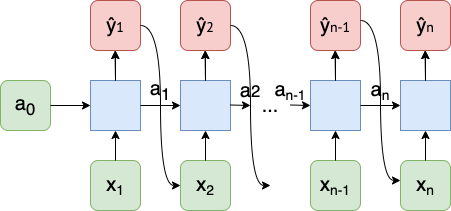
\includegraphics[width=0.7\columnwidth]{chapter07/figure-sec3/rnn_network.png}
		\centering
	\caption{Cấu trúc mạng RNN}
	\label{fig:rnn_network}
\end{figure}

Hình trên miêu tả quá trình sinh chuỗi sử dụng mạng RNN được huấn luyện sẵn. Giả sử ta huẩn luyện mạng RNN với corpus Tiếng Việt và sử dụng thơ Truyện Kiều của Nguyễn Du. Ta mong đợi mạng sau khi được huấn luyện có thể tự động sinh ra các câu thơ với phong cách Nguyễn Du.

Để cho dễ hiểu, ta giả sử corpus có 10 chữ: \textit{["Đầu", "lòng", "hai", "ả", "tố", "nga", "Thúy", "Kiều", <SOS>, <EOS>]}. Trong đó \textit{<SOS>} là start of string, \textit{<EOS>} là end of string.

Đầu tiên, ta khởi tạo trạng thái $a_0$ bằng vector 0, $x_1$ là token đầu tiên trong câu nên ta sẽ gán nó là token \textit{<SOS>} để đánh dấu sự bắt đầu của câu mới.

Thực hiện forward bước đầu, ta thu được trạng thái $a_1$ và một phân phối xác suất ở ngõ ra $\hat{y}_1$. Phân phối xác suất này cho ta biết xác suất xuất hiện của từ tiếp theo trong câu. Ví dụ, nếu phân phối xác suất ở ngõ ra $\hat{y}$ có dạng:
\begin{align*}
  \hat{y} &= [0.2, \, 0.3, \, 0.05, \, 0.05, \, 0.01, \, 0.1, \, 0.09, \, 0.05, \, 0.05, \, 0.1]
\end{align*}

Ta sẽ sử dụng phân phối này để lấy mẫu ngẫu nhiên (áp dụng giải thuật lấy mẫu nêu ở phần trên). Giải thuật này có thể cho ra bất kì từ nào trong corpus có xác suất tại $\hat{y}_1$ lớn hơn 0. Giả sử bộ lấy mẫu cho ra từ \textit{"Đầu"}, ta sẽ gán $x_2$ = \textit{"Đầu"} \, và tiếp tục dự đoán $\hat{y}_2$.

Lúc này, trạng thái $a_1$ cũng được đưa vào đầu vào trạng thái của mạng, ta tiếp tục tính được phân phối xác suất tại $\hat{y}_2$ và bộ lấy mẫu trả về kết quả từ \textit{"hai"}. Cứ tiếp tục như vậy, bộ có thể sinh ra một câu văn hoàn chỉnh như sau: \textit{"Đầu lòng hai ả tố nga <EOS>"}. Câu văn kết thúc khi \textit{<EOS>} được sinh ra.

\subsubsection{Sinh chuỗi với các từ được gợi ý}

\begin{figure}[h!]
	\centering
		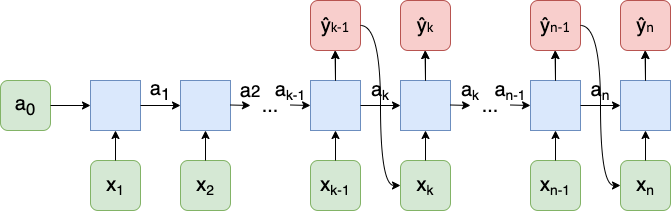
\includegraphics[width=1\columnwidth]{chapter07/figure-sec3/rnn_network2.png}
		\centering
	\caption{Cấu trúc mạng RNN sinh chuỗi với các từ được gợi ý}
\end{figure}

Để mạng RNN sinh chuỗi đúng với chủ đề mà ta muốn, ta có thể gợi ý cho mạng RNN một số từ chủ đề ban đầu và để nó tự động sinh ra các từ để hoàn thành câu.

Để làm được như vậy, ta vẫn sẽ sử dụng mạng RNN đã được huấn luyện như phần trên. Nhưng lần này, thay vì mở đầu bằng token \textit{<SOS>}, ta sẽ đưa vào $[x_1, x_2, x_3,...,x_k]$ $k$ từ đầu tiên được gợi ý.

Ví dụ ta gợi ý 2 từ \textit{"Thúy Kiều"}, ở lần forward đầu tiên, $a_0$ sẽ được gán bằng vector $0$, $x_1$ sẽ là vector của từ \textit{"Thúy"}. Mạng sẽ tính ra $\hat{y}_1$ và $a_1$. Tuy nhiên lần này ta sẽ không quan tâm đến $\hat{y}_1$, ta chỉ cần truyền $a_1$ đến ngõ vào tiếp theo của mạng. Ở lần forward thứ 2, $x_2$ sẽ là vector của từ \textit{"Kiều"}, ta tính được $\hat{y}_2$ và $a_2$. Vì \textit{"
Kiều"} là từ cuối cùng được gợi ý, nên $\hat{y}_2$ trong trường hợp này sẽ được nhận làm $x_3$ và $a_2$ sẽ được đưa đến bước tính tiếp theo. Từ đây, các từ sẽ được sinh ra cho tới khi câu được hoàn thành.

Với cách sinh chuỗi này, lượng từ gợi ý càng nhiều thì các từ sinh ra càng tự nhiên và đúng chủ đề hơn. Nguyên nhân là do mạng RNN có khả năng ghi nhớ chủ đề và trạng thái thái sẽ được điều chỉnh lại qua mỗi từ gợi ý để sinh ra các phân phối xác suất chuẩn xác hơn ở những lần sinh mẫu sau.

\subsubsection{Sinh chuỗi ở cấp độ từ và cấp độ ký tự}
Phần trên đã mô tả việc sinh mẫu ở cấp độ từ. Như ta thấy, để sinh ra các câu văn cho một ngôn ngữ nào đó, ta cần một lượng từ vựng rất lớn, vì vậy corpus cho việc sinh mẫu cũng lớn (với tiếng Anh có thể lên đến hơn 10000 từ). Đồng thời, trước khi huấn luyện, ta phải qua bước tiền xử lý \textit{word2vec} (\textit{skip-gram} hoặc \textit{CBOW} để ghi lại ngữ cảnh của từ). Đôi khi, có một khả năng từ được sinh ra là token \textit{<UNK>} (Unknown). 

Việc sinh mẫu ở cấp độ từ gây ra nhiều sự phức tạp và khó khăn, và đôi khi cho kết quả không tốt. Thay vào đó ta sẽ xem xét việc sử dụng các ký tự trong corpus thay vì các từ. Điều này cho phép chúng ta giảm bớt sự phức tạp trong việc tiền xử lý dữ liệu và giảm thiểu việc sử dụng bộ nhớ.

Để áp dụng mô hình sinh mẫu bằng ký tự, đầu tiên ta thực hiện việc thiết lập corpus cho ngôn ngữ. Ví dụ ta muốn sinh các câu văn tiếng Anh, ta sẽ phải thiết lập một corpus bao gồm:
\begin{itemize}
    \item[$-$] Các ký tự a-z và A-Z
    \item[$-$] Các số từ 0-9
    \item[$-$] Các kí tự dấu câu, dấu cách, các kí tự đặc biệt nếu có
\end{itemize}

Sau khi thiết lập được corpus, ta cần phải áp dụng các bước tiền xử lý cho các văn bản mẫu. Các bước xử lý này là các bước xử lý đơn giản bao gồm việc bỏ đi các kí tự không có trong corpus và sử dụng \textit{one-hot} vector cho từng ký tự.

Sau khi tất cả dữ liệu cho việc huấn luyện đã sẵn sàng, ta có thể thiết lập mạng RNN và bắt đầu việc huấn luyện tương tự như trên mô hình RNN ở cấp độ từ. Sau khi được huấn luyện, mô hình RNN sẽ có khả năng sinh ra các ký tự và tạo thành các đoạn văn bản có phong cách tương tự như phong cách của các văn bản huấn luyện.

Ưu điểm của việc sinh mẫu theo kí tự so với việc sinh mẫu theo từ là chất lượng văn bản được sinh ra thường sẽ tốt hơn, không sinh ra token \textit{<UNK>}, tiết kiệm bộ nhớ hơn do sử dụng corpus nhỏ, không tốn nhiều công sức cho việc tiền xử lý dữ liệu. Tuy nhiên nó có thời gian huấn luyện lâu và chi phí tính toán cao hơn do mô hình này coi mỗi kí tự là một token thay vì mỗi từ là một token như mô hình từ vựng.

Hiện nay, mô hình sinh mẫu từ từ vựng trên thực tế vẫn chiếm đa số. Tuy nhiên với sức mạnh xử lý ngày càng cao của máy tính hiện đại, người ta đang bắt đầu áp dụng các mô hình sinh mẫu dựa trên kí tự vào thực tế ngày một nhiều hơn.

\subsubsection{Các ứng dụng thực tế}
Hiện tại, việc sử dụng mạng RNN đã trở nên phổ biến trong nghiên cứu cũng như ứng dụng thực tế. Facebook, Google và các hãng công nghệ khác đã tạo ra những mô hình RNN để phục vụ cho sản phẩm của họ. Trong phần này chúng ta sẽ tìm hiểu về \textit{GPT-2}, một mạng RNN được xây dựng bởi \textit{OpenAI} và một mạng RNN được huấn luyện để sinh ra các bài báo tiếng Việt.

\textit{GPT-2} được hoàn thành vào năm 2019 bởi OpenAI. Mạng RNN này được huấn luyện với tập dữ liệu 40GB ngôn ngữ tiếng Anh bao gồm các bài báo và bình luận trên internet. Mạng này có thể cho ra các câu văn rất hoàn thiện, đúng ngữ pháp và rất tự nhiên. Do lo sợ việc sẽ có người dùng mạng RNN này để tạo nên các tin giả, tác giả của mạng đã không công bố mạng hoàn chỉnh mà chỉ đưa ra cho cộng đồng một mạng được huấn luyện với tập dữ liệu nhỏ hơn. Mặc dù mạng được công bố nhỏ hơn mạng được tạo ra trong phòng thí nghiệm nhiều lần, nhưng kết quả của nó đã rất tốt và gây ấn tượng mạnh cho giới khoa học.


Hiện tại, cấu trúc của mạng này đã được công bố, nhưng trong khuôn khổ bài viết này, chúng ta sẽ không đề cập sâu đến kiến trúc của nó. Bạn đọc có thể tham khảo thêm cách để huấn luyện mạng \textit{GPT-2} ở đây: \url{https://minimaxir.com/2019/09/howto-gpt2/}

Người ta cho mạng \textit{GPT-2} học truyện Harry Potter, sau đó cho nó một câu gợi ý (Malfoy hadn't noticed anything), và sau đây là câu chuyện được viết ra:

\begin{figure}[h!]
	\centering
		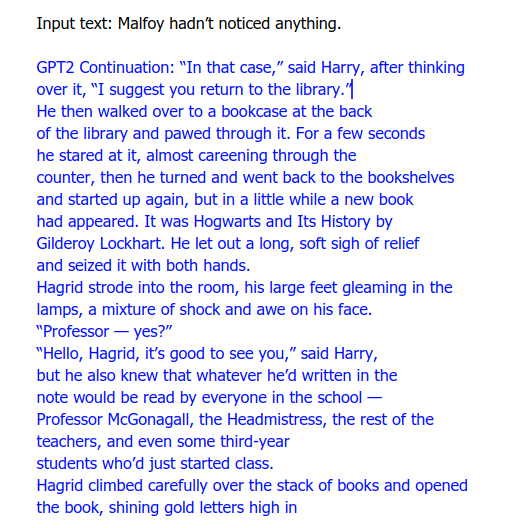
\includegraphics[width=0.7\columnwidth]{chapter07/figure-sec3/gpt-2-harrypotter.png}
		\centering
	\caption{Harry Potter được viết bởi \textit{GPT-2} [\ref{refer:23}]}
\end{figure}

Ta có thể thấy văn bản được viết đúng chính tả, ngữ pháp và có văn phong tự nhiên rất giống với tác giả J.K Rowling.

Sau đây là một ví dụ khác khi \textit{GPT-2} được huấn luyện để viết báo:

\begin{figure}[h!]
	\centering
		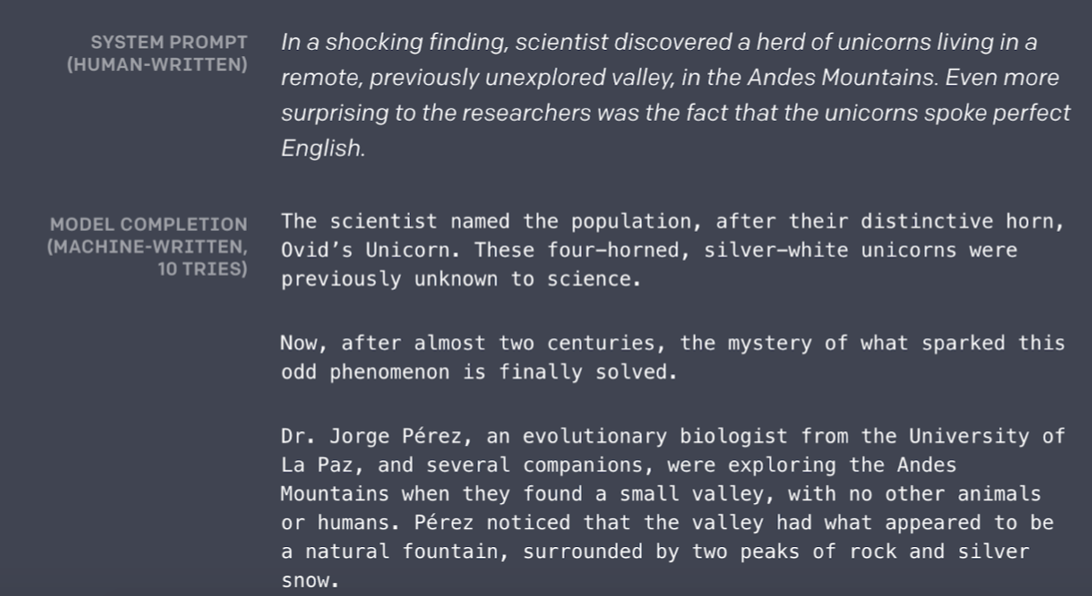
\includegraphics[width=1\columnwidth]{chapter07/figure-sec3/gpt-2-papers.png}
		\centering
	\caption{Một bài báo được viết bởi \textit{GPT-2}}
\end{figure}

Ta có thể thấy với một đoạn văn gợi ý chủ đề được viết bới con người ("In a shocking finding ..."), \textit{GPT-2} đã cho ra một bài viết có văn phong nghị luận xã hội tương tự như các bài báo nó được huấn luyện.

Tiếp theo, ta sẽ xem qua một ví dụ khác về sinh văn bản tiếng Việt. Ta lần lượt cho mạng RNN học các văn bản tin tức và Truyện Kiều, sau đây là kết quả:

\clearpage
\begin{figure}[h!]
	\centering
		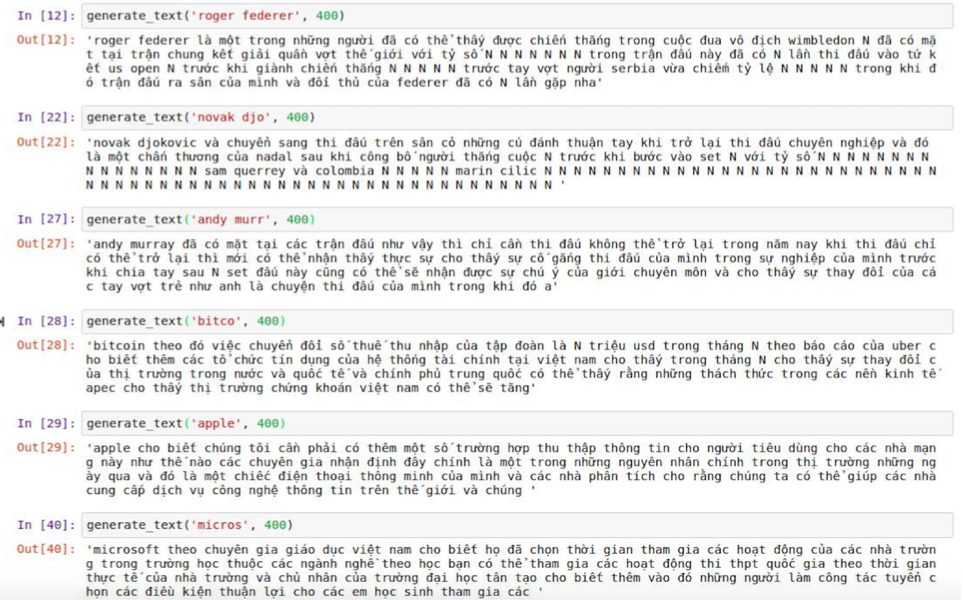
\includegraphics[width=1\columnwidth]{chapter07/figure-sec3/vnm-news.png}
		\centering
	\caption{Mạng RNN viết báo tiếng Việt}
\end{figure}
\clearpage
\begin{figure}[h!]
	\centering
		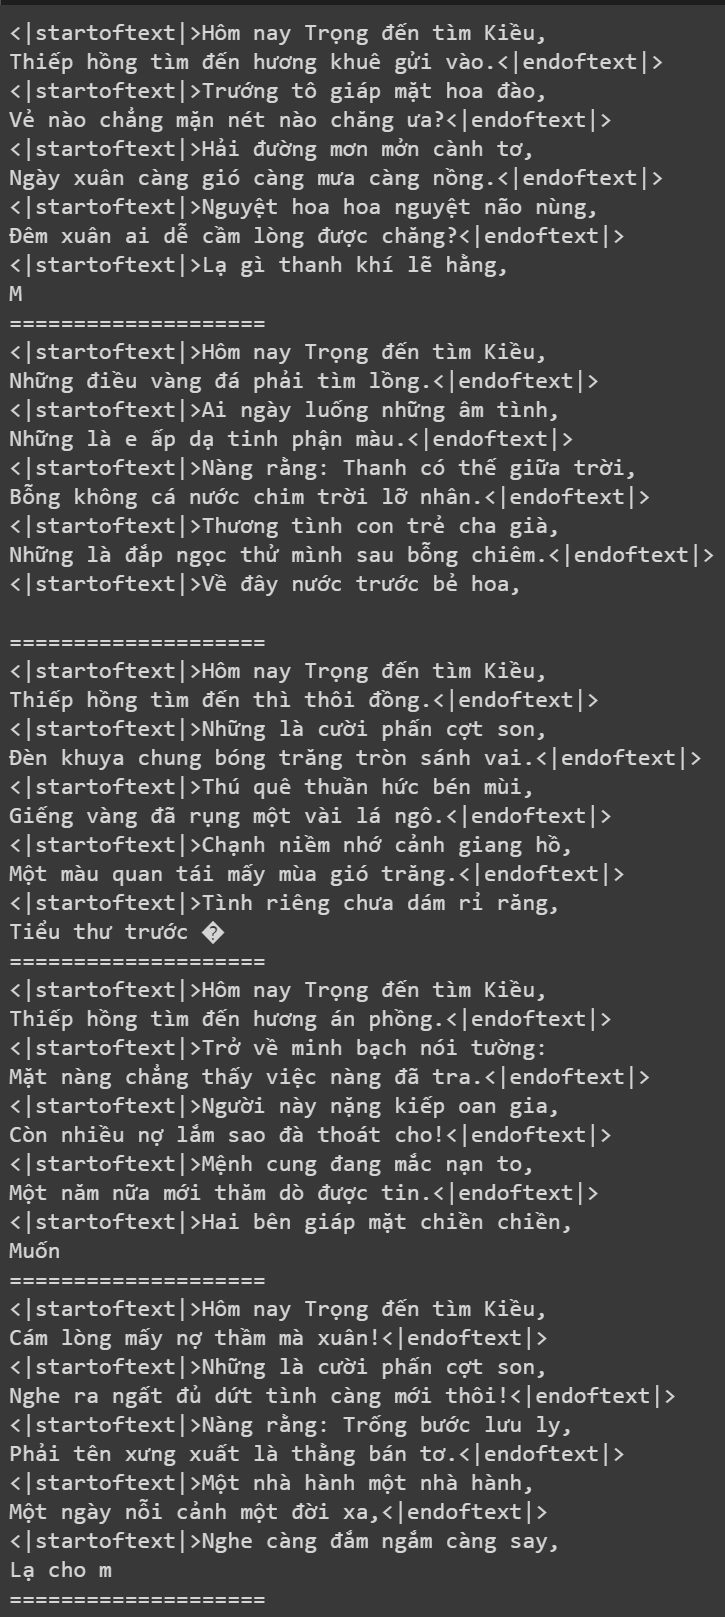
\includegraphics[width=0.64\columnwidth]{chapter07/figure-sec3/kieu.jpg}
		\centering
	\caption{Mạng RNN sáng tác truyện Kiều}
\end{figure}
